%%%%%%%%%%%%%%%%%%%%%%%%%%%%%%%%%%%%%%%%%%%%%%%%%%%%%%%%%%%%%%%%%%%%%%
%%                     Equivalence Arc
%%%%%%%%%%%%%%%%%%%%%%%%%%%%%%%%%%%%%%%%%%%%%%%%%%%%%%%%%%%%%%%%%%%%%%

\subsection{Glyph: \glyph{Equivalence arc} }\label{sec:equivalenceArc}

\glyph{Equivalence Arc} is used to represent the fact that all activities or compartments marked by a \glyph{tag} are equivalent. In an \AFm, it is used to show that an AN in a submap and another AN in the main map are equivalent.

\begin{glyphDescription}
 \glyphSboTerm Not applicable.
 \glyphOrigin Any \glyph{Activity node} (\sect{af:ANs}) or any \glyph{compartment}.
 \glyphTarget \glyph{Tag} or \glyph{Submap terminal}.
 \glyphEndPoint No symbol is used to represent the end of an \glyph{equivalence arc}.
 \end{glyphDescription}

\begin{figure}[H]
  \centering
  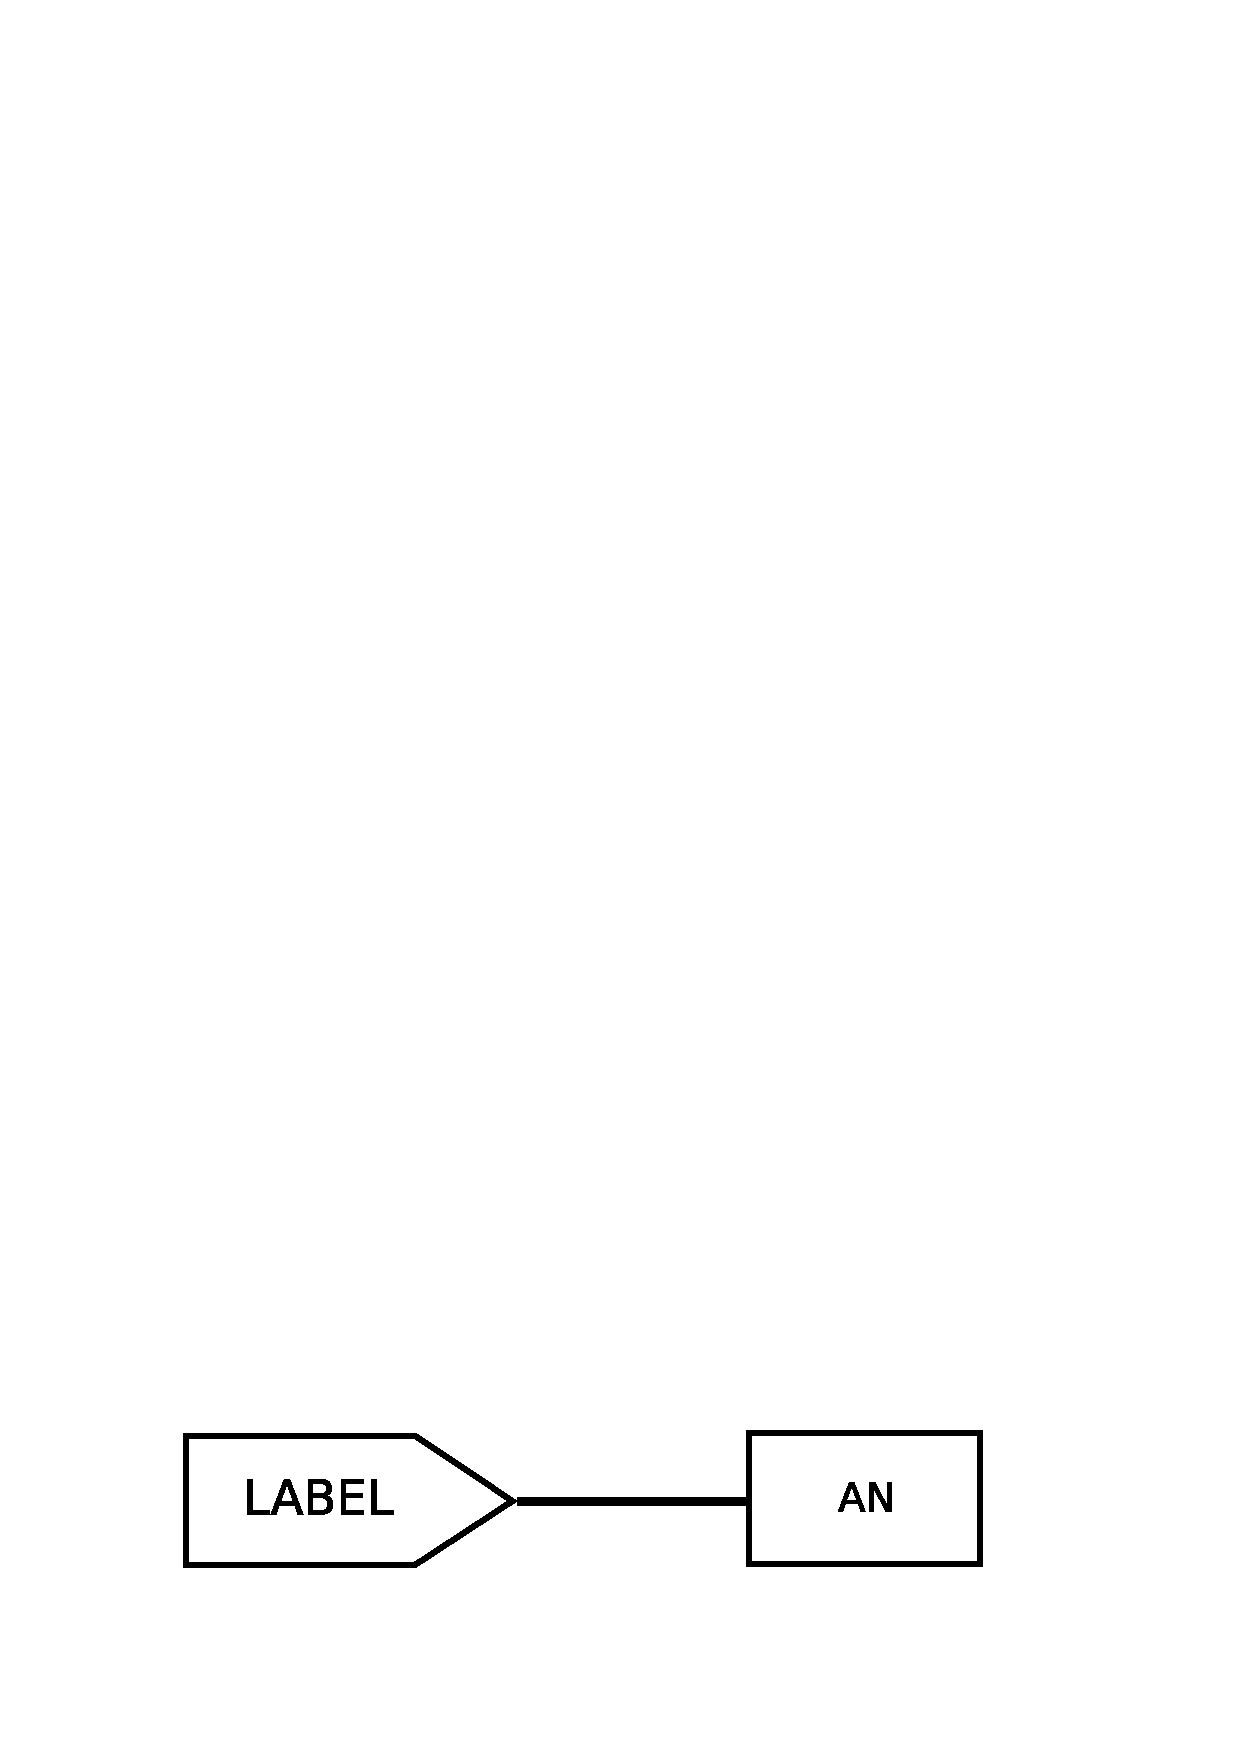
\includegraphics[scale = 0.4]{images/build/equivalence.pdf}
  \caption{The \AF glyph for \glyph{Equivalence arc}.}
  \label{fig:equivalence}
\end{figure}
